\documentclass{article}
\usepackage[utf8]{inputenc}
\pagenumbering{Roman}
\usepackage{ragged2e}
\usepackage{graphicx}
\usepackage{wrapfig}
\usepackage{tabularx}
\usepackage{array}
\usepackage{float}

\title{\huge The MAC Toolkit}
\author{Sandra Marlene Cobian Aquino \\ Guillermo Christopher Mendieta Arreola}
\date{November 3, 2026}

\begin{document}

\maketitle

\newpage

\section{Introducción}

\justifying
The Mac Toolkit es una aplicación de escritorio con estilo de videojuego con pixel art que reúne cinco proyectos: Bayesian, Heuristic, Coloring, Decision Trees y Automata. Cada proyecto se abre desde un menú que simula el inventario de un videojuego, lo que permite explorar las diferentes opciones de manera sencilla e interactiva.

El primer proyecto implementado, Bayesian Classifier, permite realizar predicciones sobre si una persona ``Camina'' o ``Conduce'', tomando como referencia su edad e ingresos. A través de la aplicación, el usuario puede observar los datos utilizados, conocer las predicciones del modelo y evaluar qué tan acertados son sus resultados. Además, puede introducir valores propios para obtener una clasificación y visualizarla en una gráfica.

El segundo proyecto, Heuristic, encuentra la ruta más corta entre dos puntos de una cuadrícula con obstáculos. El usuario puede dibujar su propio mapa, elegir entre el algoritmo de Dijkstra y dos heurísticas, y observar de forma animada cómo se explora la cuadrícula hasta encontrar la ruta.

\section{Instalación}

\begin{itemize}
  \item Windows 10 u 11.
  \item No requiere Python.
\end{itemize}

\subsection{Abrir la aplicación}

\begin{enumerate}
  \item Copiar el archivo \texttt{MacToolkit.exe} a la computadora.
  \item Hacer doble click sobre él.
  \item Esperar unos segundos.
  \item Navegar por la aplicación.
\end{enumerate}

\section{Conociendo la interfaz}

\subsection{Navegación}

La aplicación tiene tres niveles de pantallas:

\begin{enumerate}
  \item \textbf{Inicio:} pantalla principal con el botón START.
  \item \textbf{Proyectos:} menú con los cinco proyectos disponibles.
  \item \textbf{Página de cada proyecto:} Bayesian, Heuristic, Coloring,
        Decision Trees o Automata.
\end{enumerate}

Para avanzar se usa el botón \textbf{START} y las casillas de cada proyecto. Para
regresar a la pantalla anterior se usa el botón \textbf{EXIT}.

\newpage

\section{Pantalla de inicio}

Al abrir la aplicación aparece la pantalla de inicio con el título
\textbf{THE MAC TOOLKIT}, el botón \textbf{START} y dos personajes.

\begin{figure}[H]
  \centering
  
\includegraphics[width=0.8\textwidth]{capturas/01_inicio_numerada.png}
  \caption{Pantalla de inicio: (1) título, (2) botón START, (3) y (4) personajes.}
\end{figure}

\begin{itemize}
  \item Al abrir la aplicación, los personajes entran caminando desde los lados
        de la pantalla.
  \item Al pasar el mouse sobre un personaje, este levanta los brazos.
  \item Al darle click, hace una pose de fuerza durante un momento.
  \item Al dar click en \textbf{START}, los personajes saltan y se abre la página
        de proyectos.
\end{itemize}

\begin{figure}[H]
  \centering
  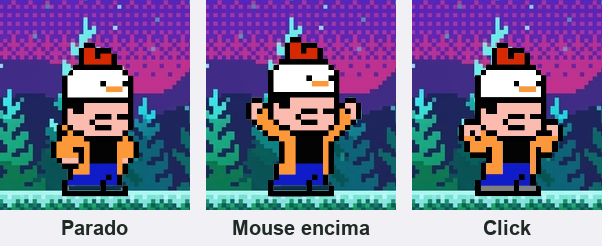
\includegraphics[width=0.6\textwidth]{capturas/02_avatar_poses.png}
  \caption{Poses del personaje: parado, con el mouse encima y al darle click.}
\end{figure}

\newpage
\section{Página de proyectos}

La página de proyectos muestra cinco casillas, cada una con un ícono y un botón
debajo:

\begin{table}[H]
  \centering
  \begin{tabular}{ll}
    \hline
    \textbf{Ícono} & \textbf{Proyecto} \\
    \hline
    Espada          & BAYESIAN \\
    Poción          & HEURISTIC \\
    Hongo           & COLORING \\
    Árbol           & DECISION TREES \\
    Reloj de arena  & AUTOMATA \\
    \hline
  \end{tabular}
  \caption{Menú de proyectos.}
\end{table}

\begin{itemize}
  \item Para entrar a un proyecto, se da click en su casilla o en el botón que
        está debajo. Al pasar el mouse, el borde de la casilla se ilumina en
        dorado.
  \item El botón \textbf{EXIT} regresa a la pantalla de inicio.
\end{itemize}

\begin{figure}[H]
  \centering
  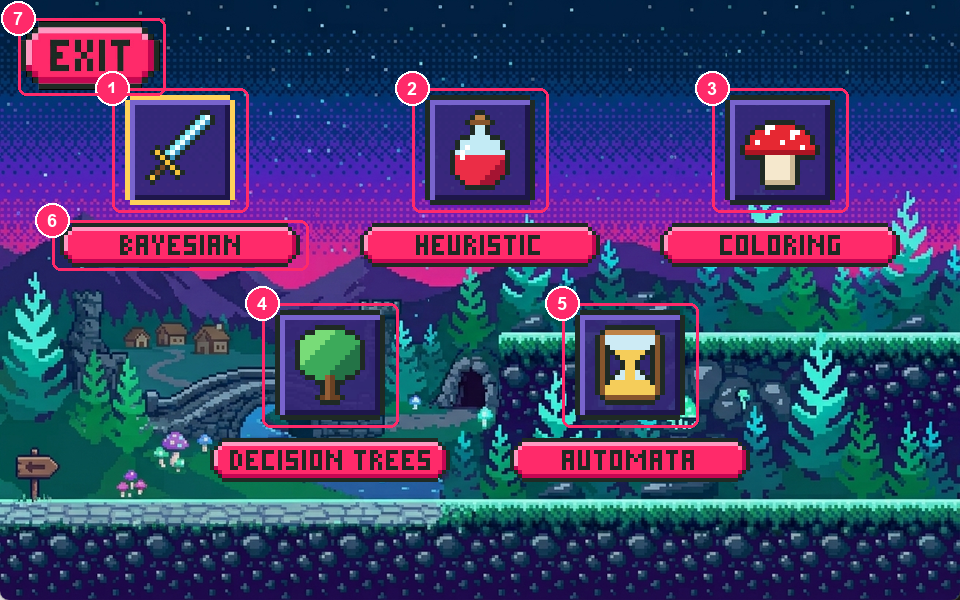
\includegraphics[width=0.8\textwidth]{capturas/04_proyectos_numerada.png}
  \caption{Página de proyectos: (1)--(5) casillas, (6) botón del proyecto,
           (7) botón EXIT.}
\end{figure}

\newpage

\section{Proyecto Bayesian}

\subsection{¿Qué hace?}

Este proyecto predice si una persona \textbf{camina} o \textbf{conduce} según su
\textbf{edad} y su \textbf{ingreso}. Para aprender, el modelo usa una encuesta de
100 personas: 80 para aprender y 20 para comprobar qué tan bien acierta.

\subsection{Elementos de la pantalla}

\begin{figure}[H]
  \centering
  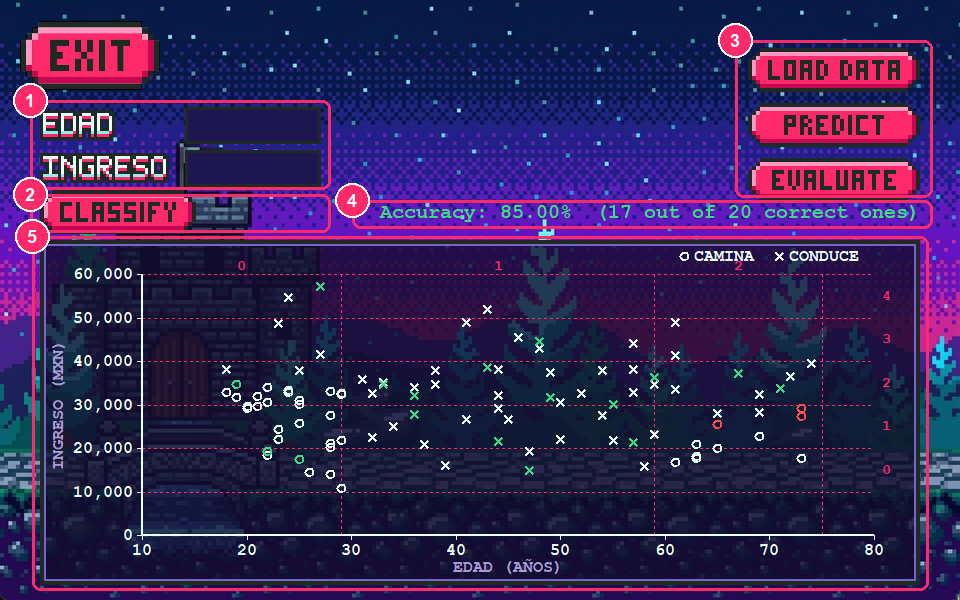
\includegraphics[width=0.8\textwidth]{capturas/05_bayesian_numerada.png}
  \caption{Elementos de la página del proyecto Bayesian.}
\end{figure}

\begin{enumerate}
  \item Campos \textbf{EDAD} e \textbf{INGRESO}.
  \item Botón \textbf{CLASSIFY} y su resultado.
  \item Botones \textbf{LOAD DATA}, \textbf{PREDICT} y \textbf{EVALUATE}.
  \item Mensajes, que aparecen arriba a la derecha de la gráfica.
  \item Gráfica de edad (eje horizontal) contra ingreso (eje vertical).
\end{enumerate}

\subsection{Paso a paso}

\paragraph{Paso 1: Cargar los datos.}

\begin{enumerate}
  \item Dar click en \textbf{LOAD DATA}.
  \item Aparecen en \textbf{blanco} los 80 datos de la encuesta que usa el modelo
        para aprender.
  \item Arriba se muestra el mensaje
        \texttt{Train: 80 registers | Test: 20 registers}.
\end{enumerate}

\begin{figure}[H]
  \centering
  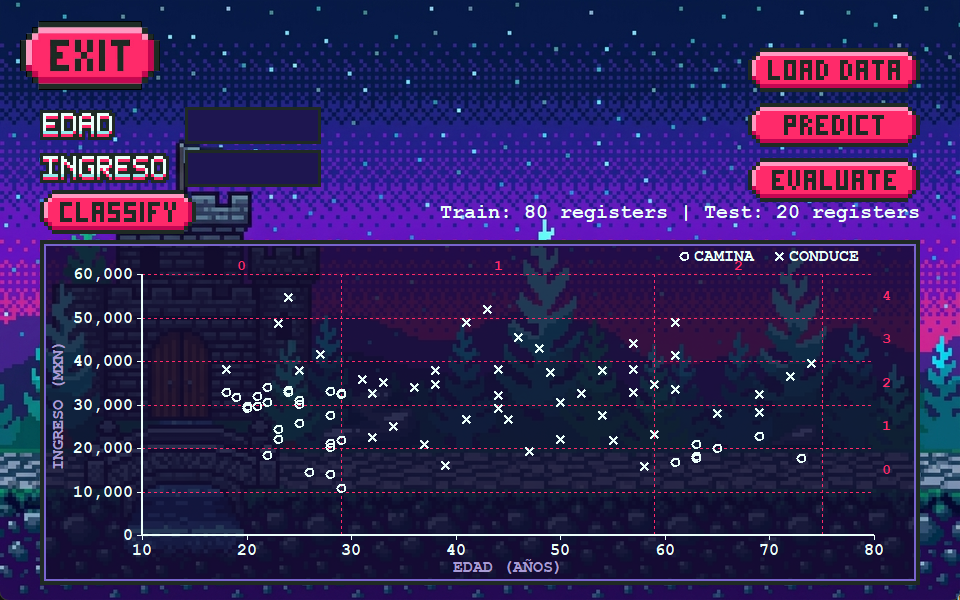
\includegraphics[width=0.8\textwidth]{capturas/06_bayesian_load_data.png}
  \caption{Datos de entrenamiento después de LOAD DATA.}
\end{figure}

\paragraph{Paso 2: Predecir.}

\begin{enumerate}
  \item Dar click en \textbf{PREDICT}.
  \item Aparecen en \textbf{amarillo} los otros 20 datos, con el símbolo de lo que
        el modelo \textit{cree} que hace cada persona: círculo si camina y cruz si
        conduce.
\end{enumerate}

\begin{figure}[H]
  \centering
  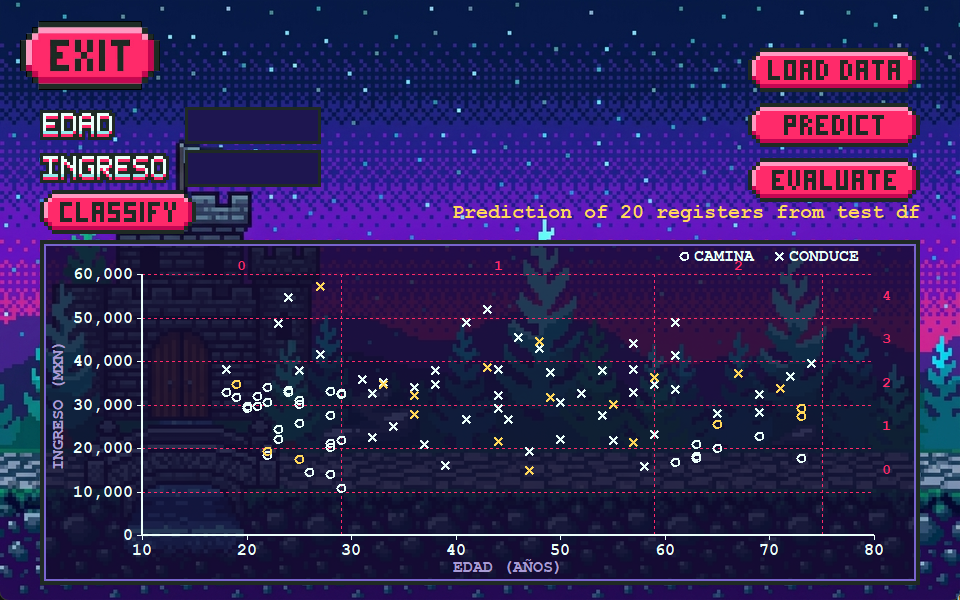
\includegraphics[width=0.8\textwidth]{capturas/07_bayesian_predict.png}
  \caption{Predicciones de los datos de prueba después de PREDICT.}
\end{figure}

\paragraph{Paso 3: Evaluar.}

\begin{enumerate}
  \item Dar click en \textbf{EVALUATE}.
  \item Los puntos amarillos cambian de color: \textbf{verde} si el modelo acertó
        y \textbf{rojo} si se equivocó.
  \item Arriba se muestra la precisión del modelo, por ejemplo:
        \texttt{Accuracy: 85.00\% (17 out of 20 correct ones)}.
\end{enumerate}

\begin{figure}[H]
  \centering
  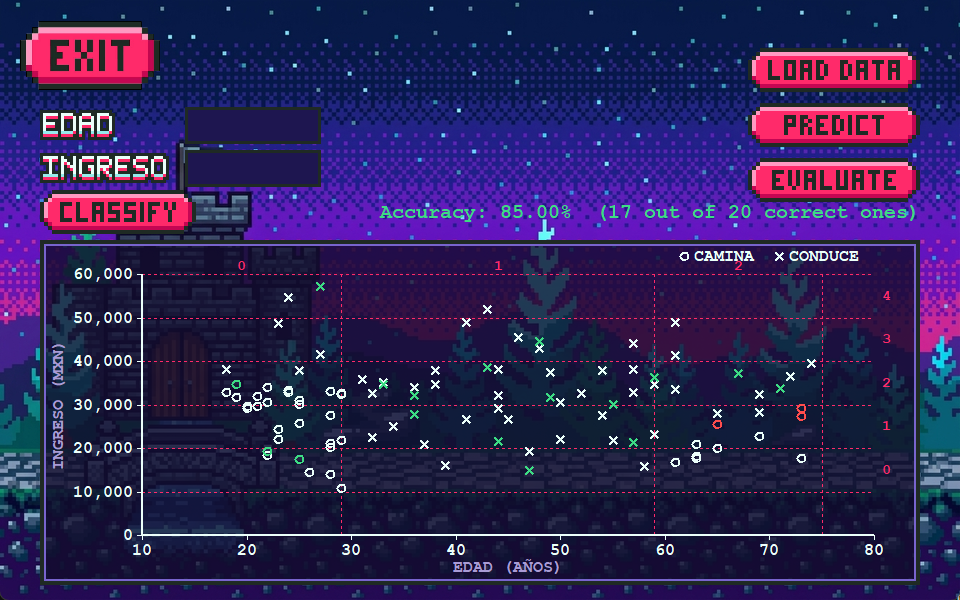
\includegraphics[width=0.8\textwidth]{capturas/08_bayesian_evaluate.png}
  \caption{Resultado de la evaluación después de EVALUATE.}
\end{figure}

\paragraph{Paso 4: Clasificar a una persona.}

\begin{enumerate}
  \item Escribir una edad en el campo \textbf{EDAD}, por ejemplo \texttt{35}.
  \item Escribir un ingreso en el campo \textbf{INGRESO}, por ejemplo
        \texttt{27000}. Se puede escribir con o sin coma.
  \item Dar click en \textbf{CLASSIFY}.
  \item Aparece un punto \textbf{azul claro} en la gráfica y, junto al botón, el
        resultado con su porcentaje, por ejemplo \textbf{Conduce (92\%)}.
\end{enumerate}

Es posible clasificar a varias personas; cada una agrega un nuevo punto azul a la
gráfica.

\begin{figure}[H]
  \centering
  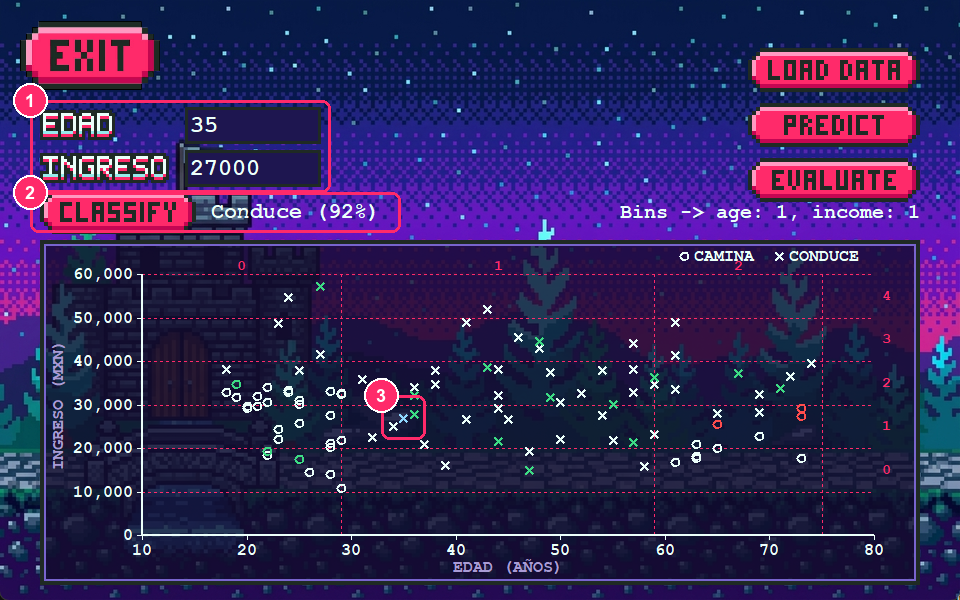
\includegraphics[width=0.8\textwidth]{capturas/09_bayesian_classify_numerada.png}
  \caption{Clasificación manual: (1) valores escritos, (2) resultado,
           (3) punto en la gráfica.}
\end{figure}

\subsection{Cómo leer la gráfica}

\begin{table}[H]
  \centering
  \small
  \begin{tabularx}{0.85\textwidth}{>{\raggedright\arraybackslash}p{4.5cm}
                                    >{\raggedright\arraybackslash}X}
    \hline
    \textbf{Símbolo o color} & \textbf{Significado} \\
    \hline
    Círculo                 & Camina \\
    Cruz                    & Conduce \\
    Blanco                  & Datos con los que aprendió el modelo \\
    Amarillo                & Predicción del modelo para los datos de prueba \\
    Verde                   & El modelo acertó \\
    Rojo                    & El modelo se equivocó \\
    Azul claro              & Persona clasificada manualmente \\
    Líneas rosas punteadas  & Límites de los rangos de edad e ingreso \\
    Números rosas           & Número de cada rango \\
    \hline
  \end{tabularx}
  \caption{Significado de los símbolos y colores de la gráfica.}
\end{table}

\newpage
\section{Mensajes y solución de problemas}

Si una acción no se puede realizar, la aplicación muestra un mensaje en rojo
arriba a la derecha de la gráfica, como en el siguiente ejemplo:

\begin{figure}[H]
  \centering
  
\includegraphics[width=\textwidth]{capturas/10_bayesian_error.png}
  \caption{Mensaje mostrado al escribir una edad fuera de rango.}
\end{figure}

\begin{table}[H]
  \centering
  \small
  \renewcommand{\arraystretch}{1.25}
  \begin{tabularx}{\textwidth}{>{\raggedright\arraybackslash}p{4.4cm}
                               >{\raggedright\arraybackslash}X
                               >{\raggedright\arraybackslash}p{3.8cm}}
    \hline
    \textbf{Mensaje o problema} & \textbf{Por qué aparece} & \textbf{Qué hacer} \\
    \hline
    \texttt{First click on LOAD DATA}
      & Se usó CLASSIFY o PREDICT antes de cargar los datos
      & Dar click en LOAD DATA \\
    \texttt{First click on PREDICT}
      & Se usó EVALUATE antes de predecir
      & Dar click en PREDICT \\
    \texttt{Age must be a number} / \texttt{Income must be a number}
      & Se escribieron letras o el campo quedó vacío
      & Escribir solo números \\
    \texttt{Out of range}
      & La edad o el ingreso están fuera de los límites
      & Usar un valor dentro del rango \\
    \texttt{Error loading the data}
      & Falta el archivo de datos
      & Volver a descargar la aplicación completa \\
    Los puntos desaparecieron
      & Se salió de la página y se volvió a entrar; la página se reinicia
      & Repetir los pasos desde LOAD DATA \\
    La aplicación tarda en abrir
      & Es normal; la aplicación se prepara al iniciar
      & Esperar unos segundos \\
    \hline
  \end{tabularx}
  \caption{Mensajes de la aplicación y cómo resolverlos.}
\end{table}

\newpage

\section{Proyecto Heuristic}

\subsection{¿Qué hace?}

Este proyecto encuentra la \textbf{ruta más corta} entre un punto de
\textbf{inicio} y un punto \textbf{final} dentro de una cuadrícula. Se dibujan
los obstáculos y la aplicación busca el camino que los rodea con el menor número
de pasos. El movimiento solo es posible hacia arriba, abajo, izquierda o derecha.

Es posible elegir entre tres formas de buscar la ruta:

\begin{table}[H]
  \centering
  \small
  \begin{tabularx}{0.85\textwidth}{>{\raggedright\arraybackslash}p{4cm}
                                    >{\raggedright\arraybackslash}X}
    \hline
    \textbf{Opción} & \textbf{Cómo busca} \\
    \hline
    Dijkstra (none) & Explora en todas direcciones por igual, sin saber dónde
                      está el final. \\
    Manhattan       & Da prioridad a las celdas más cercanas al final, contando
                      los pasos en horizontal y vertical. \\
    Euclidean       & Da prioridad a las celdas más cercanas al final, midiendo
                      la distancia en línea recta. \\
    \hline
  \end{tabularx}
  \caption{Opciones del menú HEURISTIC.}
\end{table}

Las tres opciones encuentran la ruta óptima. La diferencia está en cuántas
celdas se necesitan explorar para encontrarla.

\subsection{Elementos de la pantalla}

\begin{figure}[H]
  \centering
  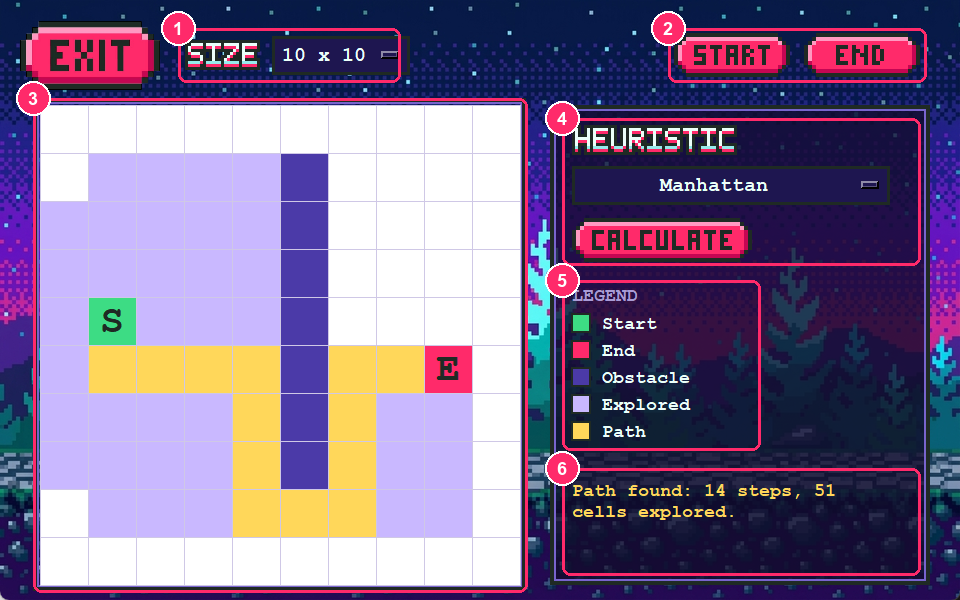
\includegraphics[width=0.8\textwidth]{capturas/12_heuristic_numerada.png}
  \caption{Elementos de la página del proyecto Heuristic.}
\end{figure}

\begin{enumerate}
  \item Menú \textbf{SIZE} para elegir el tamaño de la cuadrícula.
  \item Botones \textbf{START} y \textbf{END} para colocar el inicio y el final.
  \item Cuadrícula.
  \item Menú \textbf{HEURISTIC} y botón \textbf{CALCULATE}.
  \item Leyenda de colores.
  \item Mensajes.
\end{enumerate}

\subsection{Paso a paso}

\paragraph{Paso 1: Elegir el tamaño.}

\begin{enumerate}
  \item Dar click en el menú \textbf{SIZE}.
  \item Elegir \texttt{5 x 5}, \texttt{10 x 10}, \texttt{15 x 15} o
        \texttt{20 x 20}.
  \item La cuadrícula se crea de nuevo, vacía.
\end{enumerate}

\paragraph{Paso 2: Dibujar los obstáculos.}

\begin{enumerate}
  \item Dar click sobre una celda blanca para convertirla en obstáculo
        (\textbf{morado}).
  \item Dar click sobre un obstáculo para quitarlo.
  \item Para dibujar varios seguidos, mantener presionado el botón del mouse y
        arrastrarlo sobre la cuadrícula.
\end{enumerate}

\paragraph{Paso 3: Colocar el inicio y el final.}

\begin{enumerate}
  \item Dar click en \textbf{START} y después en una celda de la cuadrícula.
        Aparece en \textbf{verde} con la letra \textbf{S}.
  \item Dar click en \textbf{END} y después en otra celda. Aparece en
        \textbf{rosa} con la letra \textbf{E}.
  \item Para moverlos, dar click de nuevo en START o END y elegir otra celda.
\end{enumerate}

\begin{figure}[H]
  \centering
  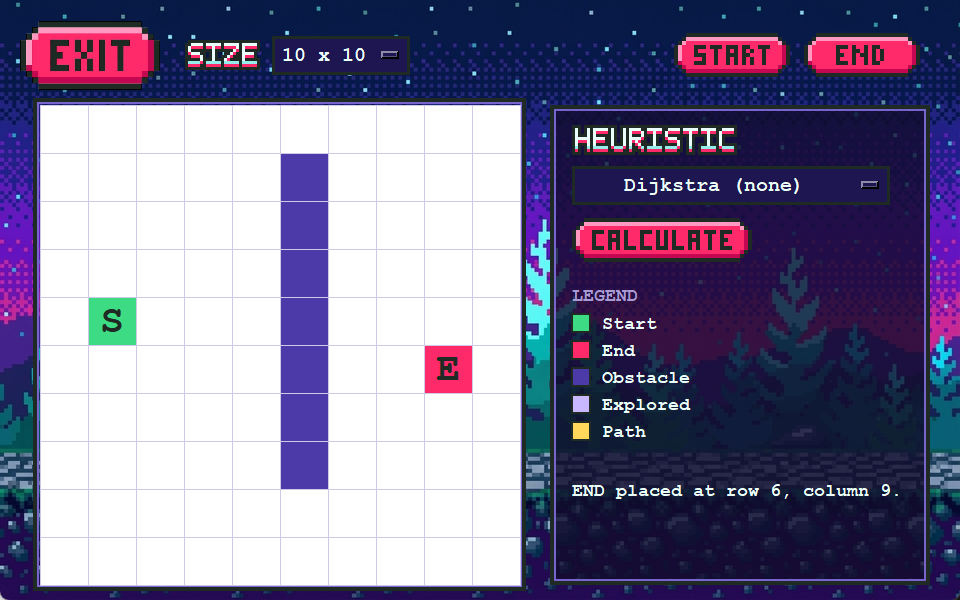
\includegraphics[width=0.8\textwidth]{capturas/13_heuristic_obstaculos.png}
  \caption{Cuadrícula con obstáculos, inicio y final.}
\end{figure}

\paragraph{Paso 4: Calcular la ruta.}

\begin{enumerate}
  \item Elegir una opción en el menú \textbf{HEURISTIC}.
  \item Dar click en \textbf{CALCULATE}.
  \item Las celdas que revisa el algoritmo se pintan poco a poco de
        \textbf{lila}.
  \item Al encontrar el final, la ruta se pinta de \textbf{amarillo}.
  \item En los mensajes aparece el resultado, por ejemplo:
        \texttt{Path found: 14 steps, 51 cells explored.}
\end{enumerate}

\begin{figure}[H]
  \centering
  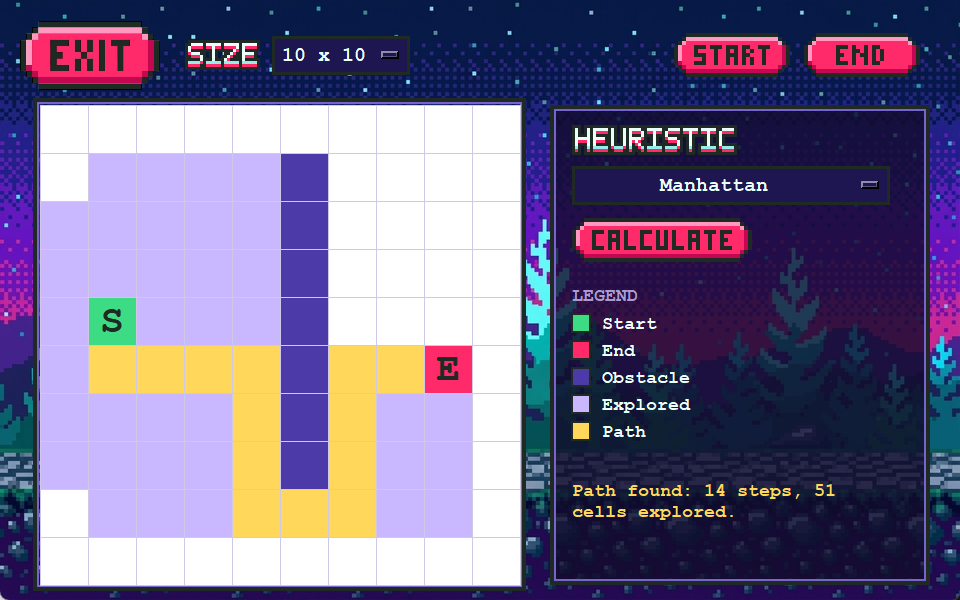
\includegraphics[width=0.8\textwidth]{capturas/14_heuristic_resultado.png}
  \caption{Celdas exploradas y ruta encontrada después de CALCULATE.}
\end{figure}

\paragraph{Paso 5: Comparar.}

Cambiar la opción del menú \textbf{HEURISTIC} y dar click de nuevo en
\textbf{CALCULATE}. La ruta anterior se borra y se calcula de nuevo con la nueva
opción. Comparar cuántas celdas se exploraron con cada una.

\subsection{Cómo leer la cuadrícula}

\begin{table}[H]
  \centering
  \small
  \begin{tabularx}{0.85\textwidth}{>{\raggedright\arraybackslash}p{4.5cm}
                                    >{\raggedright\arraybackslash}X}
    \hline
    \textbf{Color} & \textbf{Significado} \\
    \hline
    Blanco          & Celda libre \\
    Morado          & Obstáculo \\
    Verde (S)       & Inicio \\
    Rosa (E)        & Final \\
    Lila            & Celda que revisó el algoritmo \\
    Amarillo        & Ruta más corta encontrada \\
    \hline
  \end{tabularx}
  \caption{Significado de los colores de la cuadrícula.}
\end{table}

\subsection{Mensajes}

\begin{table}[H]
  \centering
  \small
  \renewcommand{\arraystretch}{1.25}
  \begin{tabularx}{\textwidth}{>{\raggedright\arraybackslash}p{4.4cm}
                               >{\raggedright\arraybackslash}X
                               >{\raggedright\arraybackslash}p{3.8cm}}
    \hline
    \textbf{Mensaje} & \textbf{Por qué aparece} & \textbf{Qué hacer} \\
    \hline
    \texttt{Place START and END first.}
      & Se dio click en CALCULATE sin colocar el inicio o el final
      & Colocar ambos con START y END \\
    \texttt{That cell is an obstacle. Choose another one.}
      & Se intentó poner el inicio o el final sobre un obstáculo
      & Elegir una celda blanca \\
    \texttt{START and END can't be the same cell.}
      & Se intentó poner el inicio y el final en la misma celda
      & Elegir otra celda \\
    \texttt{Use START or END to move this cell.}
      & Se dio click sobre el inicio o el final sin presionar antes START o END
      & Dar click en START o END y luego en la nueva celda \\
    \texttt{No path found}
      & Los obstáculos encierran el inicio o el final
      & Quitar algunos obstáculos para abrir un camino \\
    \hline
  \end{tabularx}
  \caption{Mensajes del proyecto Heuristic y cómo resolverlos.}
\end{table}

\newpage
\section{Proyectos Coloring, Decision Trees y Automata}

Estos proyectos se encuentran en desarrollo. Por ahora, al entrar se muestra la
pantalla \textbf{GAME OVER}. El botón \textbf{EXIT} regresa a la página de
proyectos.

\begin{figure}[H]
  \centering
  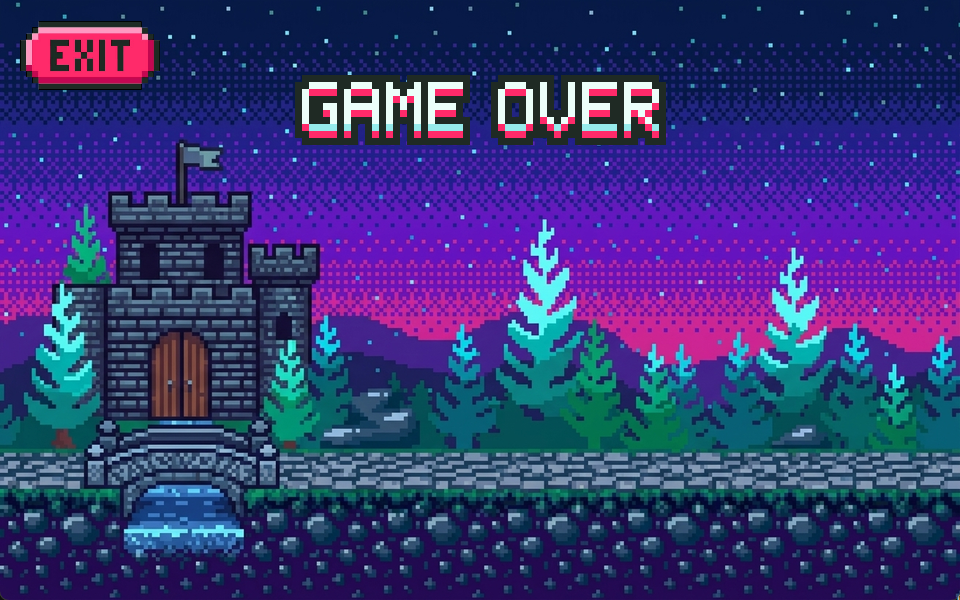
\includegraphics[width=0.8\textwidth]{capturas/11_game_over.png}
  \caption{Pantalla de los proyectos en desarrollo.}
\end{figure}

\end{document}
